\section{$n$-step Bootstrapping}
In the previous chapter we discussed one-step TD prediction, and in the chapter previous to that we discussed monte carlo methods where predictions are made based on returns at the end of the episode. In this chapter we will discuss an approach between these two, where predictions are made after $n$-steps in the future. Doing so is often more effective than either of the two previously presented approaches. 

\subsection{$n$-step TD Prediction}
The spectrum of $n$-step TD methods is summarised by Figure \ref{fig: n-step methods}. Recall from the previous chapter that our one-step return used for TD(0) was:
\begin{equation}
	G_{t:t+1} = R_{t+1} + \gamma V_t(S_{t+1})
\end{equation}
we can generalise this to the $n$-step case as follows:
\begin{equation}
	G_{t:t+n} = R_{t+1} + \gamma R_{t+2} + \cdots + \gamma^{n-1}R_{t+n} + \gamma^nV_{t+n-1}(S_{t+n})
\end{equation}
for all $n, t$ such that $n \geq 1$ and $0 \leq t \leq T - n$. All $n$-step returns can be considered approximations to the full return, truncated after $n$ steps and then corrected for the remaining missing terms by $V_{t+n-1}(S_{t+n})$. If the n-step return extends to or beyond termination then all the missing terms are taken as zero.

\begin{figure}[h!]
	\centering
	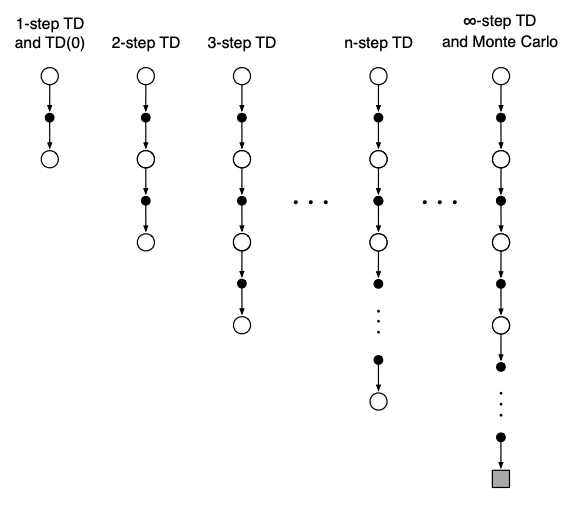
\includegraphics[width=0.7\textwidth]{/chapter7_1}
	\caption{Backup diagram for TD(0)}
	\label{fig: n-step methods}
\end{figure}\label{key}

The $n$-step return uses the value function $V_{t+n-1}$ to correct for missing rewards beyond $R_{t+n}$. An important property of $n$-step returns is that their expectation is guaranteed to be a better estimate of $v_\pi$ that $V_{t+n-1}$ in a worst-state sense i.e.:
\begin{equation}
\max_{s}|\mathbb{E}_\pi \left[G_{t:t+n} | S_t = s\right] - v_\pi(s)| \leq \gamma^n \max_{s} |V_{t+n-1}(s) - v_\pi(s)|
\end{equation}

This is called the error reduction property of $n$-step returns. Because of this, one can show formally that all $n$-step TD methods converge to t he correct predictions under appropriate conditions.

\subsection{$n$-step Sarsa}
We can extend $n$-step value function prediction to a control algorithm by incorporating the ideas of the Sarsa. Now, instead of making value function updates based on rewards received to the $t+n^{th}$ state, we select update our state-action value function $Q$ by making updates up to the $t+n^{th}$ state-action pair. The family of $n$-step Sarsa backup diagrams is shown in Figure \ref{fig: n-step sarsa methods}. The $n$-step Sarsa update is:
\begin{equation} \label{eq: n-step sarsa}
Q_{t+n}(S_t, A_t) = Q_{t+n-1}(S_t, A_t) + \alpha \left[G_{t:t+n} - Q_{t+n-1}(S_t, A_t)\right]
\end{equation}

\begin{figure}[h!]
	\centering
	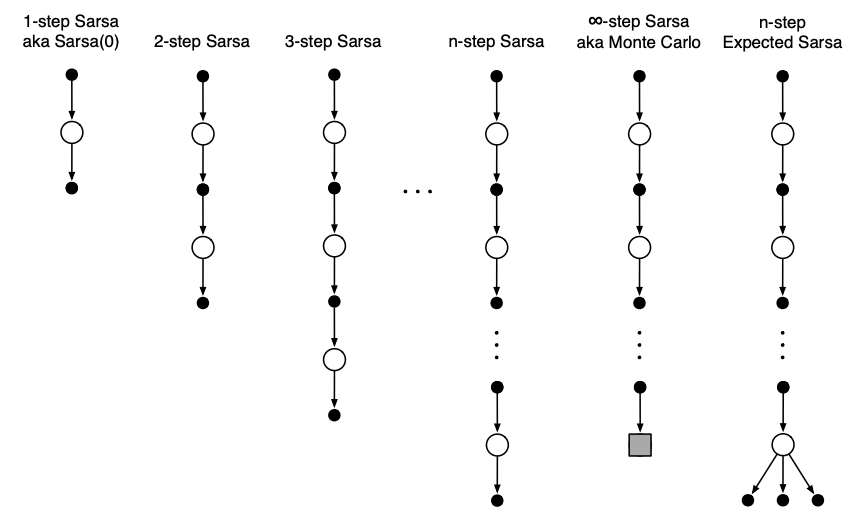
\includegraphics[width=0.7\textwidth]{/chapter7_2}
	\caption{Backup diagrams for family of $n$-step Sarsa algorithms}
	\label{fig: n-step sarsa methods}
\end{figure}

An example of why $n$-step sarsa speeds up policy learning is given in Figure \ref{fig: n-step sarsa speed up}
\begin{figure}
	\centering
	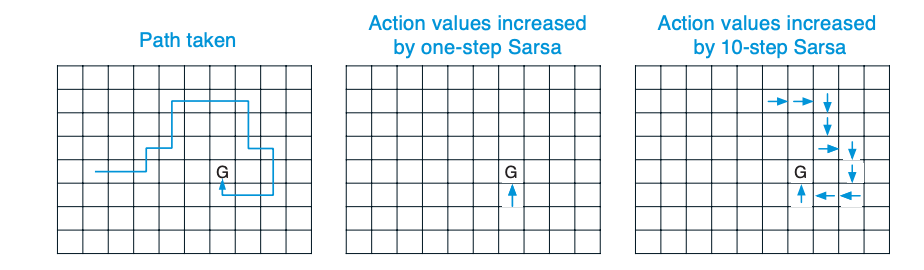
\includegraphics[width=0.8\textwidth]{/chapter7_3}
	\caption{Gridworld example of the speedup of policy learning due to the use of n-step methods. The first panel shows the path taken by an agent in a single episode, ending at a location of high reward, marked by the G. In this example the values were all initially 0, and all rewards were zero except for a positive reward at G. The arrows in the other two panels show which action values were strengthened as a result of this path by one-step and n-step Sarsa methods. The one-step method strengthens only the last action of the sequence of actions that led to the high reward, whereas the n-step method strengthens the last n actions of the sequence, so that much more is learned from the one episode.}
	\label{fig: n-step sarsa speed up}
\end{figure}

Expected Sarsa remains an important version of Sarsa because of the variance-reducing expectation. The algorithm is described as in equation \ref{eq: n-step sarsa}, but this time the expected return includes the expected value of the final value function, i.e.:
\begin{equation}
G_{t:t+n} = R_{t+1} + \cdots + \gamma^{n-1}R_{t+n} + \gamma^n \bar{V}_{t+n-1}(S_{t+n})
\end{equation}
where $\bar{V}_{t+n-1}(s)$ is the \textit{expected approximate value} of state $s$, using the estimated action values at time $t$, under the target policy:
\begin{equation}
\bar{V}_{t}(s) \doteq \sum_{a} \pi(a|s) Q_t(s,a), \; \; \text{for all} \; s \in \mathcal{S}
\end{equation}

Expected approximate values are used in developing many of the action-value method discussed hereafter. 

\subsection{$n$-step Off-policy Learning}
We can extend $n$-step learning to the off-policy case where we have a behaviour policy $b$ that creates the data and a target policy $\pi$ that we wish to update. As previously discussed, when we make updates in this way, we must weight the updates using the importance sampling ratio - equation \ref{eq: importance sampling ratio}. We can create a generalised form of the $n$-step algorithm, that works for both on-policy and off-policy cases:
\begin{equation}
Q_{t+n}(S_t, A_t) = Q_{t+n-1}(S_t, A_t) + \alpha \rho_{t+1:t+n} \left[G_{t:t+n} - Q_{t+n-1}(S_t, A_t)\right]
\end{equation}

\subsection{Per-decision Methods with Control Variates}
The off-policy methods described above may not learn as efficiently as they could. If we consider the case where the behaviour policy does not match the target policy for one of the $n$ steps used in the update, the update will go to 0 and the value function estimate will not change. Instead we can use a more sophisticated approach, that has a different definiton of the $n$-step horizon:
\begin{equation} \label{eq: off policy n step}
G_{t:h} \doteq \rho_t (R_{t+1} + \gamma G_{t+1:h}) + (1 - \rho_t)V_{h-1}(S_t)
\end{equation}

In this approach, if $\rho_t$ is zero, then instead of the target being zero and causing the estimate to shrink, the target is the same as the estimate and causes no change. Because the expected value of $\rho_t$ is 1, the expected value of the second term in equation \ref{eq: off policy n step}, called the \textit{control variate} has expected value of 0, and so does not change the update in expectation.

\subsection{Off-policy Learning Without Importance Sampling: The $n$-step Tree Backup Algorithm}
Here we will discuss off-policy learning without the need for importance sampling, conceptualised by the $n$-step Tree Backup Algorithm–Figure \ref{fig: tree-backup update}. In this tree backup update, the target now includes all rewards \textit{plus} the estimated values of the dangling action nodes hanging off the sides, at all levels. It is an update from the \textit{entire tree} of estimated action values. For each node in the tree backup diagram, we the estimated values of the non-selected actions are weighted  by their probability of being selected under our policy $\pi(A_t|S_t)$. The value of the selected action does not contribute at all at this stage, instead its probability of being selected weights the instantaneous reward of the next state \textit{and} each of the non-selected actions at the next state, which too are weighted by their probabilities of occurring as described previously. Formally, the one-step return is as follows:
\begin{equation}
G_{t:t+1} \doteq R_{t+1} + \gamma \sum_{a} \pi(a | S_{t+1}) Q_t(S_{t+1}, a)
\end{equation}

the two-step backup return (for $t < T - 1$) is described recursively as:
\begin{equation}
G_{t:t+2} \doteq R_{t+1} + \gamma \sum_{a \neq A_{t+1}} \pi(a | S_{t+1}) Q_t(S_{t+1}, a) + \gamma \pi(A_{t+1} | S_{t+1})G_{t+1:t+2}
\end{equation}

in the general case this becomes:
\begin{equation}
G_{t:t+n} \doteq R_{t+1} + \gamma \sum_{a \neq A_{t+1}} \pi(a | S_{t+1}) Q_{t+n-1}(S_{t+1}, a) + \gamma \pi(A_{t+1} | S_{t+1})G_{t+1:t+n}
\end{equation}

These returns are then used in the normal action-value update for $n$-step sarsa, as described by equation \ref{eq: n-step sarsa}.

\begin{figure}
	\centering
	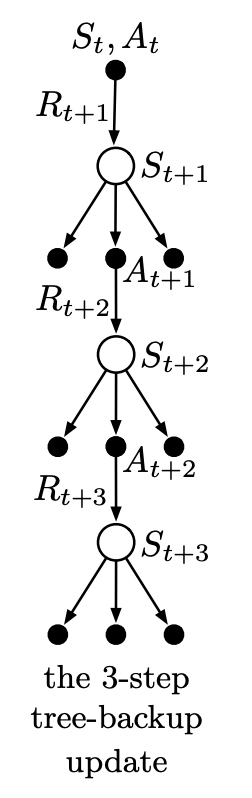
\includegraphics[width=0.15\textwidth]{/chapter7_4}
	\caption{The 3-step tree-backup update}
	\label{fig: tree-backup update}
\end{figure}

\subsection{A Unifying Algorithm: $n$-step Q($\sigma$)}
We'd like an algorithm that generalises the differences between n-step sarsa, as discussed at the beginning of this chapter, and n-step tree backup as discussed at the end of this chapter. To do so, we create a new algorithm parameter $\sigma \in [0,1)]$ that acts as a linear interpolator between the two extreme cases. This allows us to do a full, expected tree back-up in some cases, and a straight sarsa update on others, or work in the continuous region between. The family of algorithms explored in this chapter are summarised in figure \ref{fig: all chap 7 backup diagrams}:

\begin{figure}
	\centering
	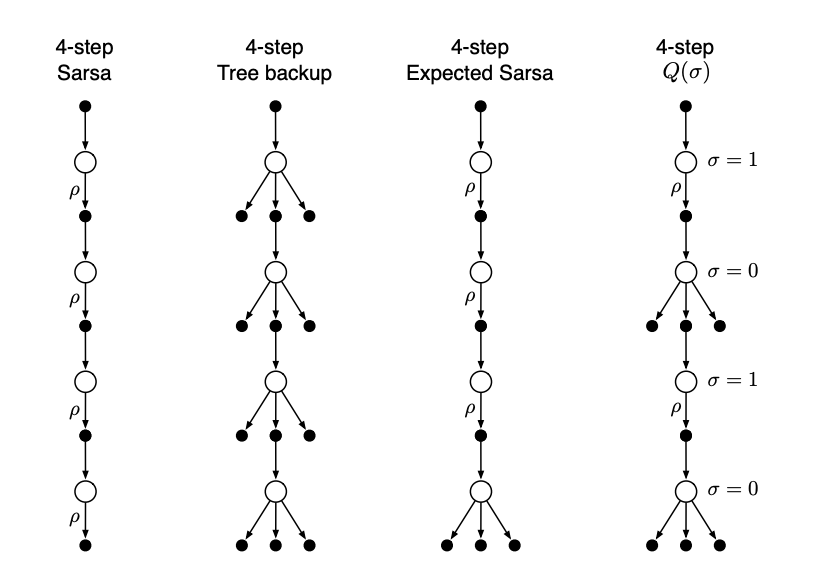
\includegraphics[width=0.75\textwidth]{/chapter7_5}
	\caption{The backup diagrams of the three kinds of n-step action-value updates considered so far in this chapter (4-step case) plus the backup diagram of a fourth kind of update that unifies them all. The label ‘$\rho$’ indicates half transitions on which importance sampling is required in the off-policy case. The fourth kind of update unifies all the others by choosing o a state-by-state basis whether to sample ($\sigma_t$ = 1) or not ($\sigma_t$= 0).}
	\label{fig: all chap 7 backup diagrams}
\end{figure}

\subsection{Key Takeaways}
\begin{itemize}
\item $n$-step TD methods lie between one-step TD methods as described in the previous chapter and full Monte Carlo backups as described in the chapter two previous. They typically perform better than either of these extremes.
\item $n$-step sarsa is an on-policy algorithm that updates state-action values based on rewards obtaining $n$ timesteps into the future following our policy $\pi$.
\item $n$-step off policy learning corrects for the failures of on-policy learning by weighting updates by the importance sampling ratio $\rho_t$ as discussed in chapter 6.
\item Variance in the off-policy $n$-step updates can be reduced using \textit{per-decision methods with control variates} that stop the value update being 0 if the behaviour policy $b$ does not match the target policy $\pi$ for any of the $n$ timesteps.
\item Finally, these methods are all more complex (expensive), and require additional memory, than one-step TD methods discussed previous.
\item We can do without importance sampling if our update is based on an expectation over each of the state-action values visited along our $n$-step trajectory. This is called the \textit{$n$-step tree backup algorithm}.
\item The continuum between all of these discussed methods can be traversed using the $n$-step Q($\sigma$) algorithm that characterised at which time steps we take full expectations and which we use only the sarsa update.
\end{itemize}